\chapter{New Material on Unsupervised Learning}
\chapterauthor{Jeff Yoshimi}

\section{Vectorized Hebb Rule}

We've seen how the Hebb rule works for scalar values. Nice and easy: if they fire together, wire together; source times target activations. The situation is the same when we vectorize the rule, but now we have activation vectors $\mathbf{a}_{\text{in}}$ and $\mathbf{a}_{\text{out}}$, and we have to find a vector operations that ``lines up'' the right components of the two vectors so that we strengthen the right ones.  Here is a preview: multiply the output activation column vector times the input row vector (the input transposed, since we assume columns to start), and out pops what we're looking for. 

% Link to new approach to matrix mult. row perspective is each component on left vector is pushed through the right vector. Col is that each right component is scanned down the left. 
So, as usual in the vector world, things end up feeling kind of backwards, we multiply output times input rather than the other way around, and there is this mysterious transpose thrown in.  But if we go back to the ``bridge'' panel of the figure above, it ends up making sense. Figure \ref{vectorizedHebb} shows the idea. I like to start in the center panel, and then (to link to the linear algebra) think of the mentally moving the output vector to the left and moving the input vector to the top. Then we have a kind of outer product representation, and all the products kind of line up in the right way. 

\begin{figure}[h]
\centering
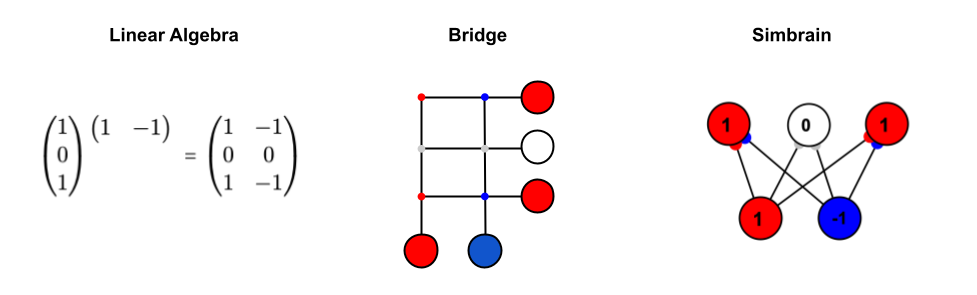
\includegraphics[width=0.9\textwidth]{images/vectorizedHebb.png}
\caption[Jeff Yoshimi.]{Using our visual conventions to conceptualized the vectorized Hebb rule,}
\label{vectorizedHebb}
\end{figure}

As a slogan: output column times input row gives you a weight matrix.

As a sanity check in the example, check the shapes. We have a $3 \times 1$ output vector times a $1 \times 2$ row vectors, which gives us a weight matrix (or weight matrix delta) in the correct shape: $3 \times 2$. This is sometimes called an outer product. So the vectorized Hebb rule is: 

\begin{eqnarray}
\label{vectorHebb}
\Delta \mathbf{W}  = \epsilon \mathbf{a}_{\text{out}} \mathbf{a}_{\text{in}} ^T
\end{eqnarray}
Remember, by default all vectors in bold face are column vectors. We are taking an $n_{out} \times 1$ column vector of output activations and matrix multiplying by a $1 \times n_{in}$ row vector input activations, to produce an $n_{out} \times n_{in}$ matrix in the same shape as the weight matrix.

Suppose we have an input vector $\mathbf{x} = (-1, 1)$, and an output vector $\mathbf{y} = (1,0,1)$ and all the weights are zero, and our learning rate is 1.
\begin{equation*}
\epsilon = 1 \; \; \; \; \\
\mathbf{a}_{\text{in}} = \begin{bmatrix} -1 \\ 1 \end{bmatrix} \\ 
\; \; \mathbf{a}_{\text{out}} = \begin{bmatrix} 1 \\ 0 \\ 1 \end{bmatrix}
\end{equation*}

We compute the new weight values using equation \eqref{vectorHebb}:
\begin{align*}
\Delta \mathbf{W}  = 1
\begin{bmatrix} 1 \\ 0 \\ 1 \end{bmatrix} 
\begin{bmatrix} -1 & 1 \end{bmatrix} 
= \begin{bmatrix} 1 \cdot -1 & 1 \cdot 1 \\ 0 \cdot -1 & 0 \cdot 1 \\ 1 \cdot -1 & 1 \cdot 1 \end{bmatrix} 
= \begin{bmatrix} -1 & 1 \\ 0 & 0 \\  -1 & 1  \end{bmatrix}
\end{align*}

% This example does not match the pic!
So we get

\begin{align*}
\mathbf{W} + \Delta \mathbf{W}  =
\begin{bmatrix} 0 & 0 \\ 0 & 0 \\  0  & 0  \end{bmatrix} +
\begin{bmatrix} -1 & 1 \\ 0 & 0 \\  -1 & 1  \end{bmatrix} =
\begin{bmatrix} -1 & 1 \\ 0 & 0 \\  -1 & 1  \end{bmatrix}
\end{align*}

Iterate again (assuming we are clamping the nodes; if we weren't the output activations would also be changing) and get


\begin{align*}
\mathbf{W} + \Delta \mathbf{W}  =
\begin{bmatrix} -1 & 1 \\ 0 & 0 \\  -1 & 1  \end{bmatrix} +
\begin{bmatrix} -1 & 1 \\ 0 & 0 \\  -1 & 1  \end{bmatrix} =
\begin{bmatrix} -2 & 2 \\ 0 & 0 \\  -2 & 2  \end{bmatrix}
\end{align*}

Keep iterating and the entries at the top and bottom right will explode to positive infinity, and the top and bottom right will explode to negative infinity. This can be seen graphically in the Simbrain neuron array representation.